% Chapter Template

\chapter{A first insight in the scanning behaviour of presocial blow fly larvae} % Main chapter title

\label{Chapter3} % Change X to a consecutive number; for referencing this chapter elsewhere, use \ref{ChapterX}

\lhead{Chapitre 3. \emph{A first insight in the scanning behaviour of presocial blow fly larvae}} % Change X to a consecutive number; this is for the header on each page - perhaps a shortened title

Julien \textsc{Boulay}\up{a,b}, Cécile \textsc{Betremieux}\up{a}, Valéry \textsc{Hédouin}\up{a} and Damien \textsc{Charabidzé}\up{a}

\up{a} Univ. Lille, CHU Lille, EA 7367 - UTML - Unité de Taphonomie Médico-Légale, Lille, France\\
\up{b} Université Libre de Bruxelles, Unit of Social Ecology, Brussels, Belgium\\


Article publié dans \emph{Physiological Entomology}, DOI: 10.1111/phen.12117.\\


\cleardoublepage

%----------------------------------------------------------------------------------------
%	SECTION 1
%----------------------------------------------------------------------------------------

\section{Abstract}
Aggregation of necrophagous larvae has several benefits: the sharing of salivary enzymes (exodigestion), temperature regulation, protection from predators and parasites, etc. and is well developed in blow flies (Diptera: Calliphoridae). This study focuses on the aggregation mechanism used by the necrophagous larvae of \textit{Lucilia sericata} Meigen, the common green bottle fly. The ability of single larva to detect and follow a signal (trail) created by conspecifics is investigated initially. A circular ring is drawn in a Petri dish where twenty starved larvae have crawled for a period of 30 min. A naïve (test) larva is then placed in the dish and video-tracked. Naïve larvae are able to detect the boundaries of the larvae-crawled area and stay preferentially within this conspecific-marked zone. In a second step, the orientation of larvae by scanning, a dedicated, ground-signal detection behaviour of dipteran larvae, is analysed. Four experimental conditions are tested: control, presence of food, conspecifics, and food + conspecifics. When conspecifics have been previously present in a given area, the scanning behaviour by naïve larvae in this area decreases (both in number and frequency of scans). Accordingly, scanning by necrophagous larvae of \textit{L. sericata} should be considered not only as locomotion behaviour but also as a potential way to detect signals from conspecifics for the purpose of aggregation. The chemical composition of the attractant(s), the behavioural effects (attraction or retention) and the implication of larval signalling in the aggregation process are new fields to explore.

\emph{Keywords:} aggregation - chemo-detection - self-organization - sensory organs - trail-follwing.

\clearpage

%----------------------------------------------------------------------------------------
%	SECTION 2
%----------------------------------------------------------------------------------------
	\section{Introduction}
Aggregation, or interattraction, is a common behaviour that occurs in many biological systems \cite{krause_living_2002}. With regard to necrophagous species, the costs and benefits of aggregation by blow fly larvae have been identified and discussed by Ives (1991) and more recently by \citet{rivers_physiological_2011}. One main advantage is the capacity of large larval masses to locally modify some of the biotic and abiotic factors of their ecosystem, leading to faster larval development. The most well-known benefit of aggregation in necrophagous larvae  is the local elevation of temperature inside aggregates, called the \textit{larval-mass effect} or more familiarly \textit{maggot-mass effect} \citep{slone_thermoregulation_2007, huckesfeld_feel_2011, rivers_physiological_2011, charabidze_larval-mass_2011}. This heat generation accelerates the development of blow flies larvae, and thus decreases the time spent by larvae on carrion \citep{heaton_quantifying_2014, johnson_effect_2014}. Gregarious behaviour also offers protection from predators and parasites, cooperation for digestion, and an increase in food assimilation (reviewed by \citet{rivers_physiological_2011}). Accordingly, gregarization appears to be a key behaviour in these species, which is especially remarkable because larval masses are self-organized structures: each larva has only a local perception of its close environment and (re)acts for itself \cite{camazine_self-organization_2001}.     
Such social organization requires at least a basic communication system between individuals \cite{camazine_self-organization_2001}. In many social insect species, such as Lepidoptera or Hymenoptera, larval aggregations are mediated by tactile and/or chemical cues (see examples in \citet{wertheim_pheromone-mediated_2005} and \citet{costa_other_2006}). However, only a few studies have investigated the mechanisms underlying the collective behaviour of blow fly larvae \citep{rivers_physiological_2011, boulay_evidence_2013}. In a recent study, the present research group \cite{boulay_evidence_2013} highlighted for the first time the existence of a signal  deposited or left passively by \textit{Lucilia sericata} larvae on the substrate over which they were crawling: these chemical cues were shown to have an attractive/retentive effect on conspecifics \cite{boulay_evidence_2013}. The present study focuses on the behavioural response of \textit{L. sericata} larvae to this signal, and particularly with regard to orientation mechanisms.

\citet{green_organization_1983} describe five elementary behaviours thought to be shared by all cyclorrhaphous dipteran larvae (i.e., species where the imago emerges from the pupal case by pushing a lid or a circular seal). These are, locomotion, turning, burrowing, rearing and bending. The authors define rearing as the raising and trembling of the head and first thoracic segments, whereas bending is described as the lateral flexing of the head and anterior segments \cite{green_organization_1983}. In other words, rearing occurs in a vertical axis and does not directly affect larval trajectory, whilst bending is laterally oriented. Accordingly, \citet{green_organization_1983} assume that bending is mainly associated with changing direction (i.e., turning) during locomotion. However, observations made in this laboratory (J. Boulay and D. Charabidzé, unpublished observations) strongly suggest that larvae may also use bending to detect the chemical signals around them and to orientate accordingly. Indeed, the anterior part of the larva’s body is the location of most of the sensory organs: Calliphoridae larvae have twelve photoreceptors (Bolwig’s organ) \cite{hinnemann_see_2010}, one olfactory and one gustatory organ \citep{chu-wang_fine_1971, cobb_what_1999,chu-wang_fine_1971-1} all located in the anterior section. Bending could therefore be involved in local signal detection and should be regarded as a scanning, i.e., \textit{a mechanism by which animals move their receptors, and sometimes their bodies or appendages, so as to capture information from the environment efficiently} \cite{bell_searching_1990}. Such a behaviour has been reported for many insect species during foraging, or when searching for conspecifics, refugees or mates \cite{bell_searching_1990}. 

To test this hypothesis, the present study first analyses the ability of \textit{L. sericata} larvae to detect and follow a track previously crawled by conspecifics (Larval trail experiment). It then focuses on the scanning behaviour, which is hypothesized to be involved in the detection of the larval signal. To test the hypothesis, the scanning behaviour of \textit{L. sericata} third-instar larvae in analysed under four different experimental conditions: control, conspecific larval signal, food, and larval signal + food together \cite{boulay_evidence_2013}. According to this hypothesis, an increase of scanning behaviour should be observed in the absence of larval signal, demonstrating active searching for the conspecific’s signal (i.e. chemotaxis \cite{gomez-marin_active_2011}). 

%----------------------------------------------------------------------------------------
%	SECTION 3
%----------------------------------------------------------------------------------------
	\section{Material and Methods}
%----------------------------------------------------------------------------------------
%	SUBSECTION 1
%----------------------------------------------------------------------------------------    
        	\subsection{Insect rearing}
The experiments were performed on \textit{L. sericata} larvae that were obtained from rearing colonies (Lille, France). Adults were reared at ambient temperature (25 $\pm$ 2 \up{o}C) under natural light  and fed ad libitum with caster sugar and water. Beginning with the adult fly emergence (day 0), fresh minced beef liver was added for seven days (day 7) to provide the proteins necessary for vitellogenesis. After five days with no food, liver was provided again to trigger egg-laying (day 12). Eggs were placed on breeding substrate (100 g of fresh minced beef liver) at 17 $\pm$ 0.5 \up{o}C (day 13). Five-to-six-day-old larvae (day 18–19, corresponding to young third instars, 10 $\pm$ 2 mm long) were used for experiments \cite{grassberger_effect_2001}. During the experiments, the temperature of the set-up was maintained at 25 $\pm$ 1 \up{o}C in a thermostatic chamber.         
    
%----------------------------------------------------------------------------------------
%	SUBSECTION 2
%----------------------------------------------------------------------------------------   
			\subsection{Larval trail experiment}
This experiment was designed to test the ability of \textit{L. sericata} larvae to follow a track created by conspecifics (i.e., a trail). The setup consists of a Petri dish (diameter: 18.5 cm; surface: 268.60 cm\up{2}; Figure \ref{fig:setup}) lined with a wet paper towel (humidified with distilled water) covering the arena surface. Two smaller Petri dishes were used to circumscribe a ring (internal diameter: 5 cm, external diameter: 4.75 cm; thick: 2 cm, surface: 37.11 cm\up{2}; Figure \ref{fig:setup}). Under the ‘Control’ condition, no deposit was made in this ring. The larval trail condition was obtained with twenty starved larvae (cleaning and starving took place for 4 h in wet pine-wood dust; a time sufficient to obtain larvae with empty crops \cite{charabidze_discontinuous_2013}) crawling in the ring area for 30 min to create the Marked Zone (MZ; Figure \ref{fig:setup}). After 30 min, these twenty larvae and the two small Petri dishes were removed. A naïve (test) larva was placed in the centre of the arena (Centre Zone (CZ): 19.63 cm\up{2}; Figure \ref{fig:setup}) in the dark and video recorded using an infrared camera (Kamatec, Kam-HWI-SH-7204). The results were analysed with Ethovision 8.0 XT software (Noldus, Netherlands): trials started when the test larvae exited the Centre Zone for the first time and were stopped when individuals were outside the Marked Zone for at least 1 min or when they had reached the wall of the arena. Twenty replicates were performed for each condition. 

\begin{figure}[ht]
	\centering
		
\includegraphics[width=0.9 \textwidth]{Figures/fig1.png}
		\rule{35em}{0.5pt}
	\caption[Setup]{Apparatus used for analyzing behavioural responses to the attractive signal from necrophagous larvae of the Green bottle fly, \textit{Lucilia sericata} (Control and Marked trials). Third-instar \textit{L. sericata} larvae were placed in the Centre Zone (CZ). Trials started when individuals entered in the Marked Zone (MZ) and stopped when larvae stayed more than 1 min completely in the Outer Zone (OZ).}
	\label{fig:setup}
\end{figure}

\clearpage
%----------------------------------------------------------------------------------------
%	SUBSECTION 2
%----------------------------------------------------------------------------------------   
			\subsection{Study of the scanning behaviour}
This experiment was designed to measure the scanning response according to larval signal. During scanning, the larva stopped and moved the anterior part of its body back and forth laterally (described in \citet{green_organization_1983}). The experimental set-up was a circular arena 9 cm in diameter as in \citet{boulay_evidence_2013}. Test larvae were isolated in wet pine-wood dust for 30 min prior to the experiments to remove any traces of their former breeding substrate (beef liver). A disc of clean paper towel covering the whole surface of the Petri dish was first humidified homogenously with 1.5 mL of distilled water. The ‘Control’ (C) consisted of no deposit on this paper (only the presence of distilled water). The ‘Food’ condition (F) consisted of 200$\mu$L of a solution containing 3 g of mixed beef liver diluted in 50 mL of distilled water. The solution was deposited using a micropipette such that the food solution was spread over the entire arena. The ‘Larvae’ condition (L) consisted of the signal created by ten larvae moving freely within the arena for 10 min and removed before the start of the trial. These signal-depositing larvae were previously starved and cleaned for 4 h in wet pine-wood dust (time sufficient to obtain larvae with empty crops \cite{charabidze_discontinuous_2013} to eliminate food odours acquired from the breeding substrate \cite{boulay_evidence_2013}. The ‘Larvae + Food’ condition (L + F) consisted of the deposition in the arena of both the larval signal and the food substrate (in that order). Twenty replicates were performed for each condition and individuals were followed for 5 min. Behavioural observations were video recorded using a digital camera (Bosch Dinion LTC0355) and analysed with Ethovision 8.0 XT software (Noldus, The Netherlands). Mean absolute meander/tortuosity, which is defined as the change in direction of movement of an individual relative to the distance (i.e., the amount of turning per unit distance) was used to describe the changes in larval orientation \cite{granchietti_fruit_2012} (Absolute Meander = |$\frac{Turn angle}{Distance moved}$|; \cite{noldus_ethovision:_2001}). The encoding of scanning behaviour was made from the video recording using sequenceR (a free interface developed by M. Hervé and available online (http://www.maximeherve.com/r-statistiques/sequencer)) implemented in R software \cite{r_development_core_team_r:_2008}. The number of scanning motions was noted for each experimental condition. 
Larval path visualisations were obtained by leaving individuals free to move on wet ground with no deposit for a few minutes. The paths were photographed using a smartphone (IPhone 5C; 8 Mpx, Apple Inc.), and edited using Adobe Photoshop CC 14.2 (Adobe Systems). The images illustrated clearly the environmental exploration of each individual larva.

%----------------------------------------------------------------------------------------
%	SUBSECTION 3
%----------------------------------------------------------------------------------------   
			\subsection{Statistical analysis}
Because the attractive signal experimental data were not normally distributed, non-parametric statistical tests (Mann-Whitney) were used to compare mean time and mean distance travelled in each zone by larvae in Control and Marked conditions. Then, bilateral tests (u$_{\alpha}$ = 1.96 for d.f. = 1; if u $>$ u$_{\alpha}$ it is considered to be significant) were used to compare the proportion of time spent in each zone (CZ, MZ and OZ) between Control and Marked conditions.
Also, because directional movement and scanning behaviour data were not normally distributed, non-parametric tests (Kruskall-Wallis, Dunn and Mann-Whitney) were used to compare larvae trajectories in all conditions and to test the effect of substrates on scanning behaviour \cite{zar_biostatistical_2010}. All tests were performed using GraphPad InStat version 3.06 for Windows. The level of significance $\alpha$ was set at 0.05.
            
%----------------------------------------------------------------------------------------
%	SECTION 4
%----------------------------------------------------------------------------------------
	\section{Results}   
    
%----------------------------------------------------------------------------------------
%	SUBSECTION 1
%----------------------------------------------------------------------------------------   
			\subsection{Setup analysis}    
This study was designed with regard to previous work from this laboratory focusing on the larval signal \cite{boulay_evidence_2013} as well as personal observations of larval scanning behaviour. First, the signal-following ability of larvae (larval trail experiment) was studied. Then, to test the hypothesis that scanning behaviour may be involved in such signal detection, the nature and quantification of scanning behaviour were explored under three relevant (natural) conditions and a blank control.

The larval instars used during the study were young third-instars. With this type of instar, sensory responses as previously observed did not differ from those of second-instars \cite{cobb_what_1999}, and their size (length) was large enough to permit tracking of larvae using trajectometry software (Ethovision 8.0 XT, Noldus). Individual larvae were followed under infrared wavelengths, thus avoiding any visible light stress \cite{hinnemann_see_2010}. Larvae were cleaned using wet pine-wood as in a study by \citet{boulay_evidence_2013}. This method could be inefficient in removing all food traces, but has been tested using larval signals on one half vs. food on the other half. In this experiment, larvae spent significantly more time in the food zone \cite{boulay_evidence_2013}. In another binary choice experiment between food + larval signal vs. food individuals are observed to stay preferentially in the food + signal zone (J. Boulay, unpublished observations). These results demonstrate the existence of the 'larval signal' exists, and that its retentive effect differs from signals based on food only. Accordingly, the cleaning method that was used to remove food traces from the cuticles of larvae appears to be effective.

The proportion of scanning movements observed during 5 min of recording decreased in all four conditions between the first minute (mean $\pm$ SD; Control: 0.3 $\pm$ 0.25; Food: 0.33 $\pm$ 0.27; Larvae: 0.21 $\pm$ 0.17; Larvae + Food: 0.21 $\pm$ 0.23) and the last minute (Control: 0.11 $\pm$ 0.16; Food: 0.08 $\pm$ 0.11; Larvae: 0.17 $\pm$ 0.18; Larvae + Food: 0.14 $\pm$ 0.19). Thus, a decision was made to analyse scanning behaviour only during the first minute of the experiments: as from previous observations and mean larval velocity, this first minute was sufficient for larvae to explore the entire arena \citep{charabidze_effect_2008, boulay_evidence_2013}.

%----------------------------------------------------------------------------------------
%	SUBSECTION 2
%----------------------------------------------------------------------------------------   
			\subsection{Larval trail experiment}  
Larval signals had a retentive effect. When conspecific larvae had been formerly present in the setup, test larvae spent significantly more time in the marked zone than those in the Control condition (mean $\pm$ SD; Control: 16.1 $\pm$ 13 s; Marked: 108.9 $\pm$ 125 s; U = 29, P $<$ 0.0001). Larval trajectories in Control condition were in straight lines with no about-turns or visible foraging (Figure \ref{fig:trail}). Accordingly, the mean distance travelled by individuals in the experimental setup was shorter in the Control condition than in the Marked condition (mean $\pm$ SD; Control: 6 $\pm$ 3 cm; Marked: 22.4 $\pm$ 21 s; U = 30, P $<$ 0.0001). Furthermore, in the absence of a signal (i.e., the Control condition), larvae never returned to the Centre Zone (CZ); they crawled straight away from centre to the outside of the arena (Figure \ref{fig:trail}). On the other hand, larvae placed in the setup marked by larval signal clearly detected the Marked Zone (MZ) and stayed preferentially within it (Fig. 2). Under these conditions, the larval trajectories were more sinuous and many larvae were able to follow the boundaries of the MZ (Figure \ref{fig:trail}). From a more quantitative point of view, the proportion of time spent in CZ and MZ during the Marked condition was significantly higher than in the Control condition (Marked vs. Control: for CZ, u = 7.58, P $<$ 0.001; for MZ, u = 14.14, P $<$ 0.001; Figure \ref{fig:proportion}). In the Control condition assays, larvae spent significantly more time in the Outer Zone (OZ) than during the Marked condition assays (for OZ, u = 27.98, P $<$ 0.001; Figure \ref{fig:proportion}).            

\begin{figure}[ht]
	\centering
		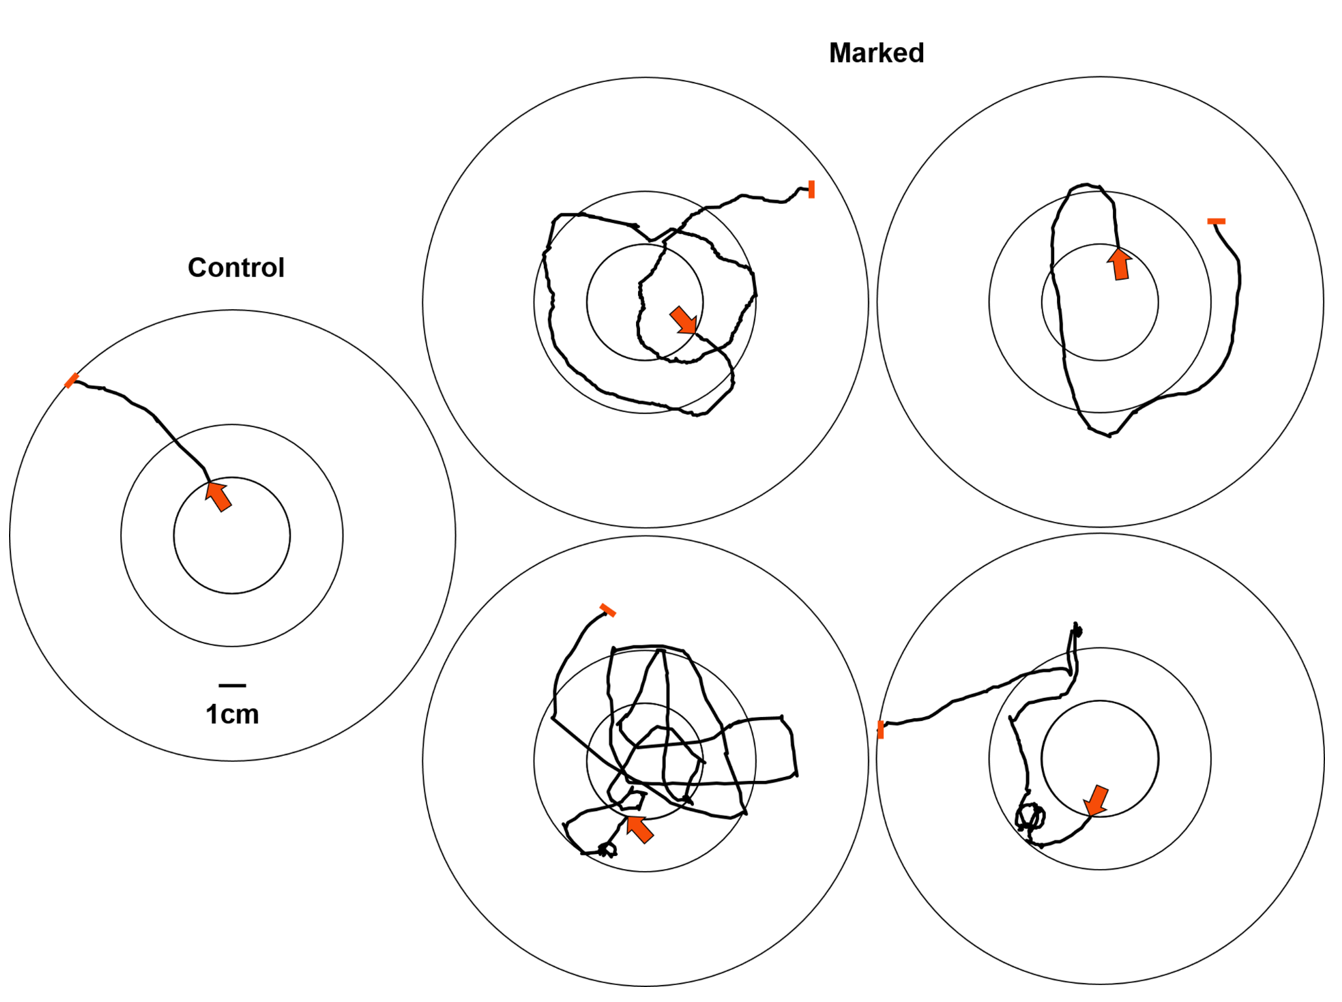
\includegraphics[width=0.9 \textwidth]{Figures/fig2.png}
		\rule{35em}{0.5pt}
	\caption[Trail]{Tracks of five \textit{Lucilia sericata} larvae during different attractive signal experiments (one Control and four Marked trials). The apparatus was comprised of three zones, a Centre Zone (the circle in the center), a Marked Zone (represented by the ring; marked by twenty starved larvae for 30 min; for Control trials this zone was unmarked), and an Outer Zone. The start point of each bioassay (trial) is represented by the arrow and the end-point by the small line. The trajectory pattern that was observed in the Control trials was the same for all of the other trials.}
	\label{fig:trail}

\end{figure}

\begin{figure}[ht]
	\centering
		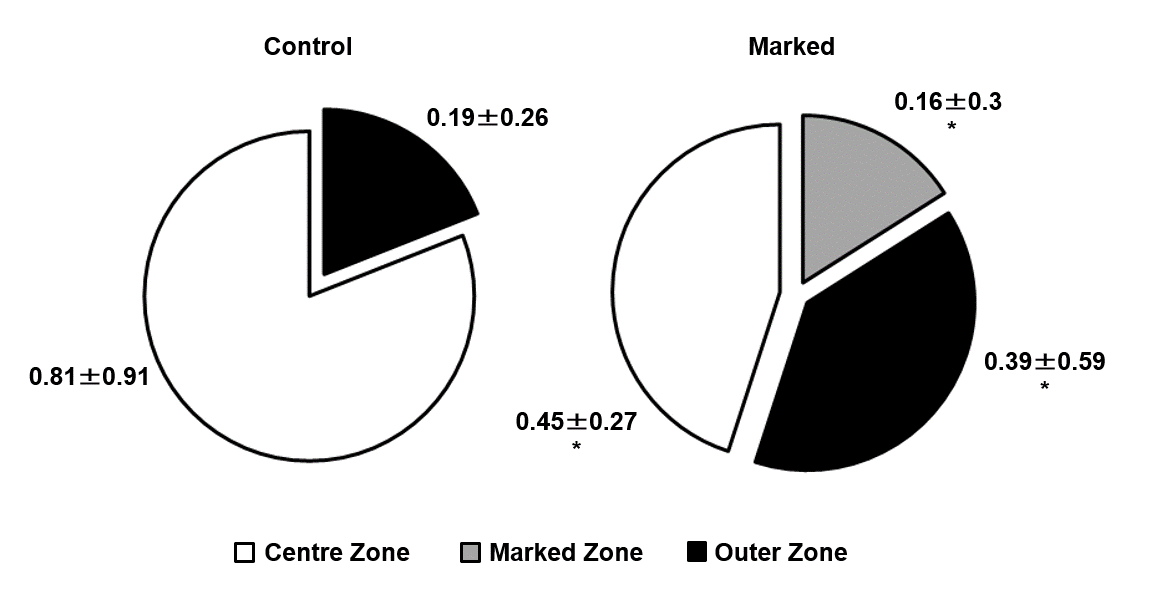
\includegraphics[width=0.9 \textwidth]{Figures/fig3.png}
		\rule{35em}{0.5pt}
	\caption[Proportion]{Mean proportion of time ($\pm$SD; n = 20) spent by \textit{Lucilia sericata} larvae in each of the behavioural trial zones. The asterisks (*) show significant differences between Control and Marked trials for each of the zones using bilateral tests \\(u$_{\alpha}$ = 1.96 for d.f. = 1).}
	\label{fig:proportion}
\end{figure}    
    
\clearpage

%----------------------------------------------------------------------------------------
%	SUBSECTION 3
%----------------------------------------------------------------------------------------   
			\subsection{Study of the scanning behaviour}  
The absolute meander was significantly higher in Signal conditions (Larvae, Food and Larvae + Food conditions) than in Control conditions, meaning that larvae had trajectories that were more tortuous when a signal was present in the arena (KW = 34.5, P $<$ 0.001). No significant differences were observed for the absolute meander between Signal conditions (Dunn’s tests: L vs. F: P $>$ 0.05; L vs. L + F: P $>$ 0.05; F vs. L + F: P $>$ 0.05).

The mean number of scanning movements varied according to test signals. Larvae scanned significantly more in the Control and Food conditions than in Larvae and Larvae + Food conditions (C vs. L: U = 81.5 P $<$ 0.01; C vs. L + F: U = 74, P $<$ 0.001; F vs. L: U = 121.5, P $<$ 0.05; F vs. L + F: U = 83, P $<$ 0.01; Figure \ref{fig:boxplot}). No significant difference was observed between the Control and Food conditions (C vs. F: U = 163.5, P $>$ 0.1; Figure \ref{fig:boxplot} ) and Larvae and Larvae + Food conditions (L vs. L + F: U = 142.5, P $>$ 0.1; Figure \ref{fig:boxplot}) again showing that scanning was decreased in the presence of the larval signal.

The larval signal also increased the time between two successive scannings: this time was significantly higher in Larvae and Larvae + Food conditions than in Control and Food conditions (C vs. L: U = 1341.5, P $<$ 0.05; C vs. L + F: U = 900.5, P $<$ 0.01; F vs. L: U = 1086, P $<$ 0.05; F vs. L + F: U = 728.8, P $<$ 0.01; Figure \ref{fig:boxplot}). As for the number of scans, the time between two successive scannings did not differ between Control and Food conditions (U = 2832.5, P $>$ 0.1; Figure \ref{fig:boxplot}) and between Larvae and Larvae + Food conditions (U = 585.5, P $>$ 0.1; Figure \ref{fig:boxplot}). 
The larval path clearly showed the places where individuals scanned (Figure \ref{fig:scan}). During their exploratory behavioural movements, larvae have intertwined locomotion and scanning (Figure \ref{fig:scan}). 
            
\begin{figure}[ht]
	\centering
		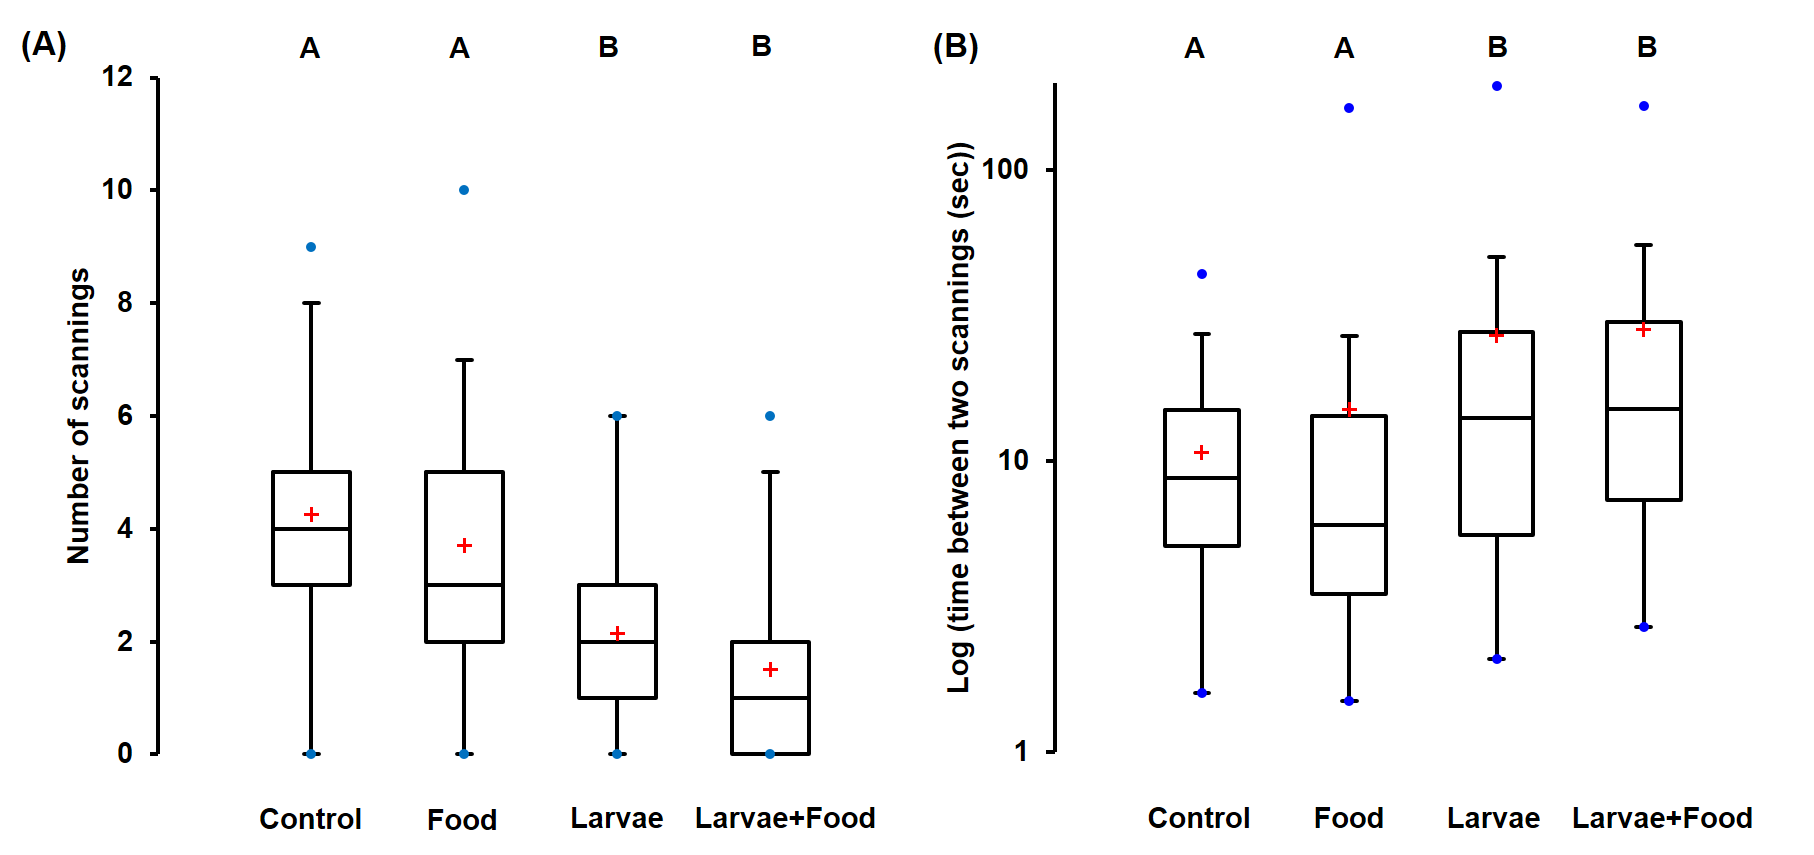
\includegraphics[width=0.9 \textwidth]{Figures/fig4.png}
		\rule{35em}{0.5pt}
	\caption[Boxplot]{(A) Boxplots of number of scannings performed by \textit{Lucilia sericata} larvae in each experimental conditions during the first minute of the experiment (n = 20, letters show significant differences in Mann-Whitney’s tests). (B) Boxplots of time (s) between two scannings of \textit{L. sericata} larvae in each experimental conditions during the first minute of experiment (n = 20, letters show significant differences in Mann-Whitney’s tests). Crosses represent the means.}
	\label{fig:boxplot}
\end{figure}

\begin{figure}[ht]
	\centering
		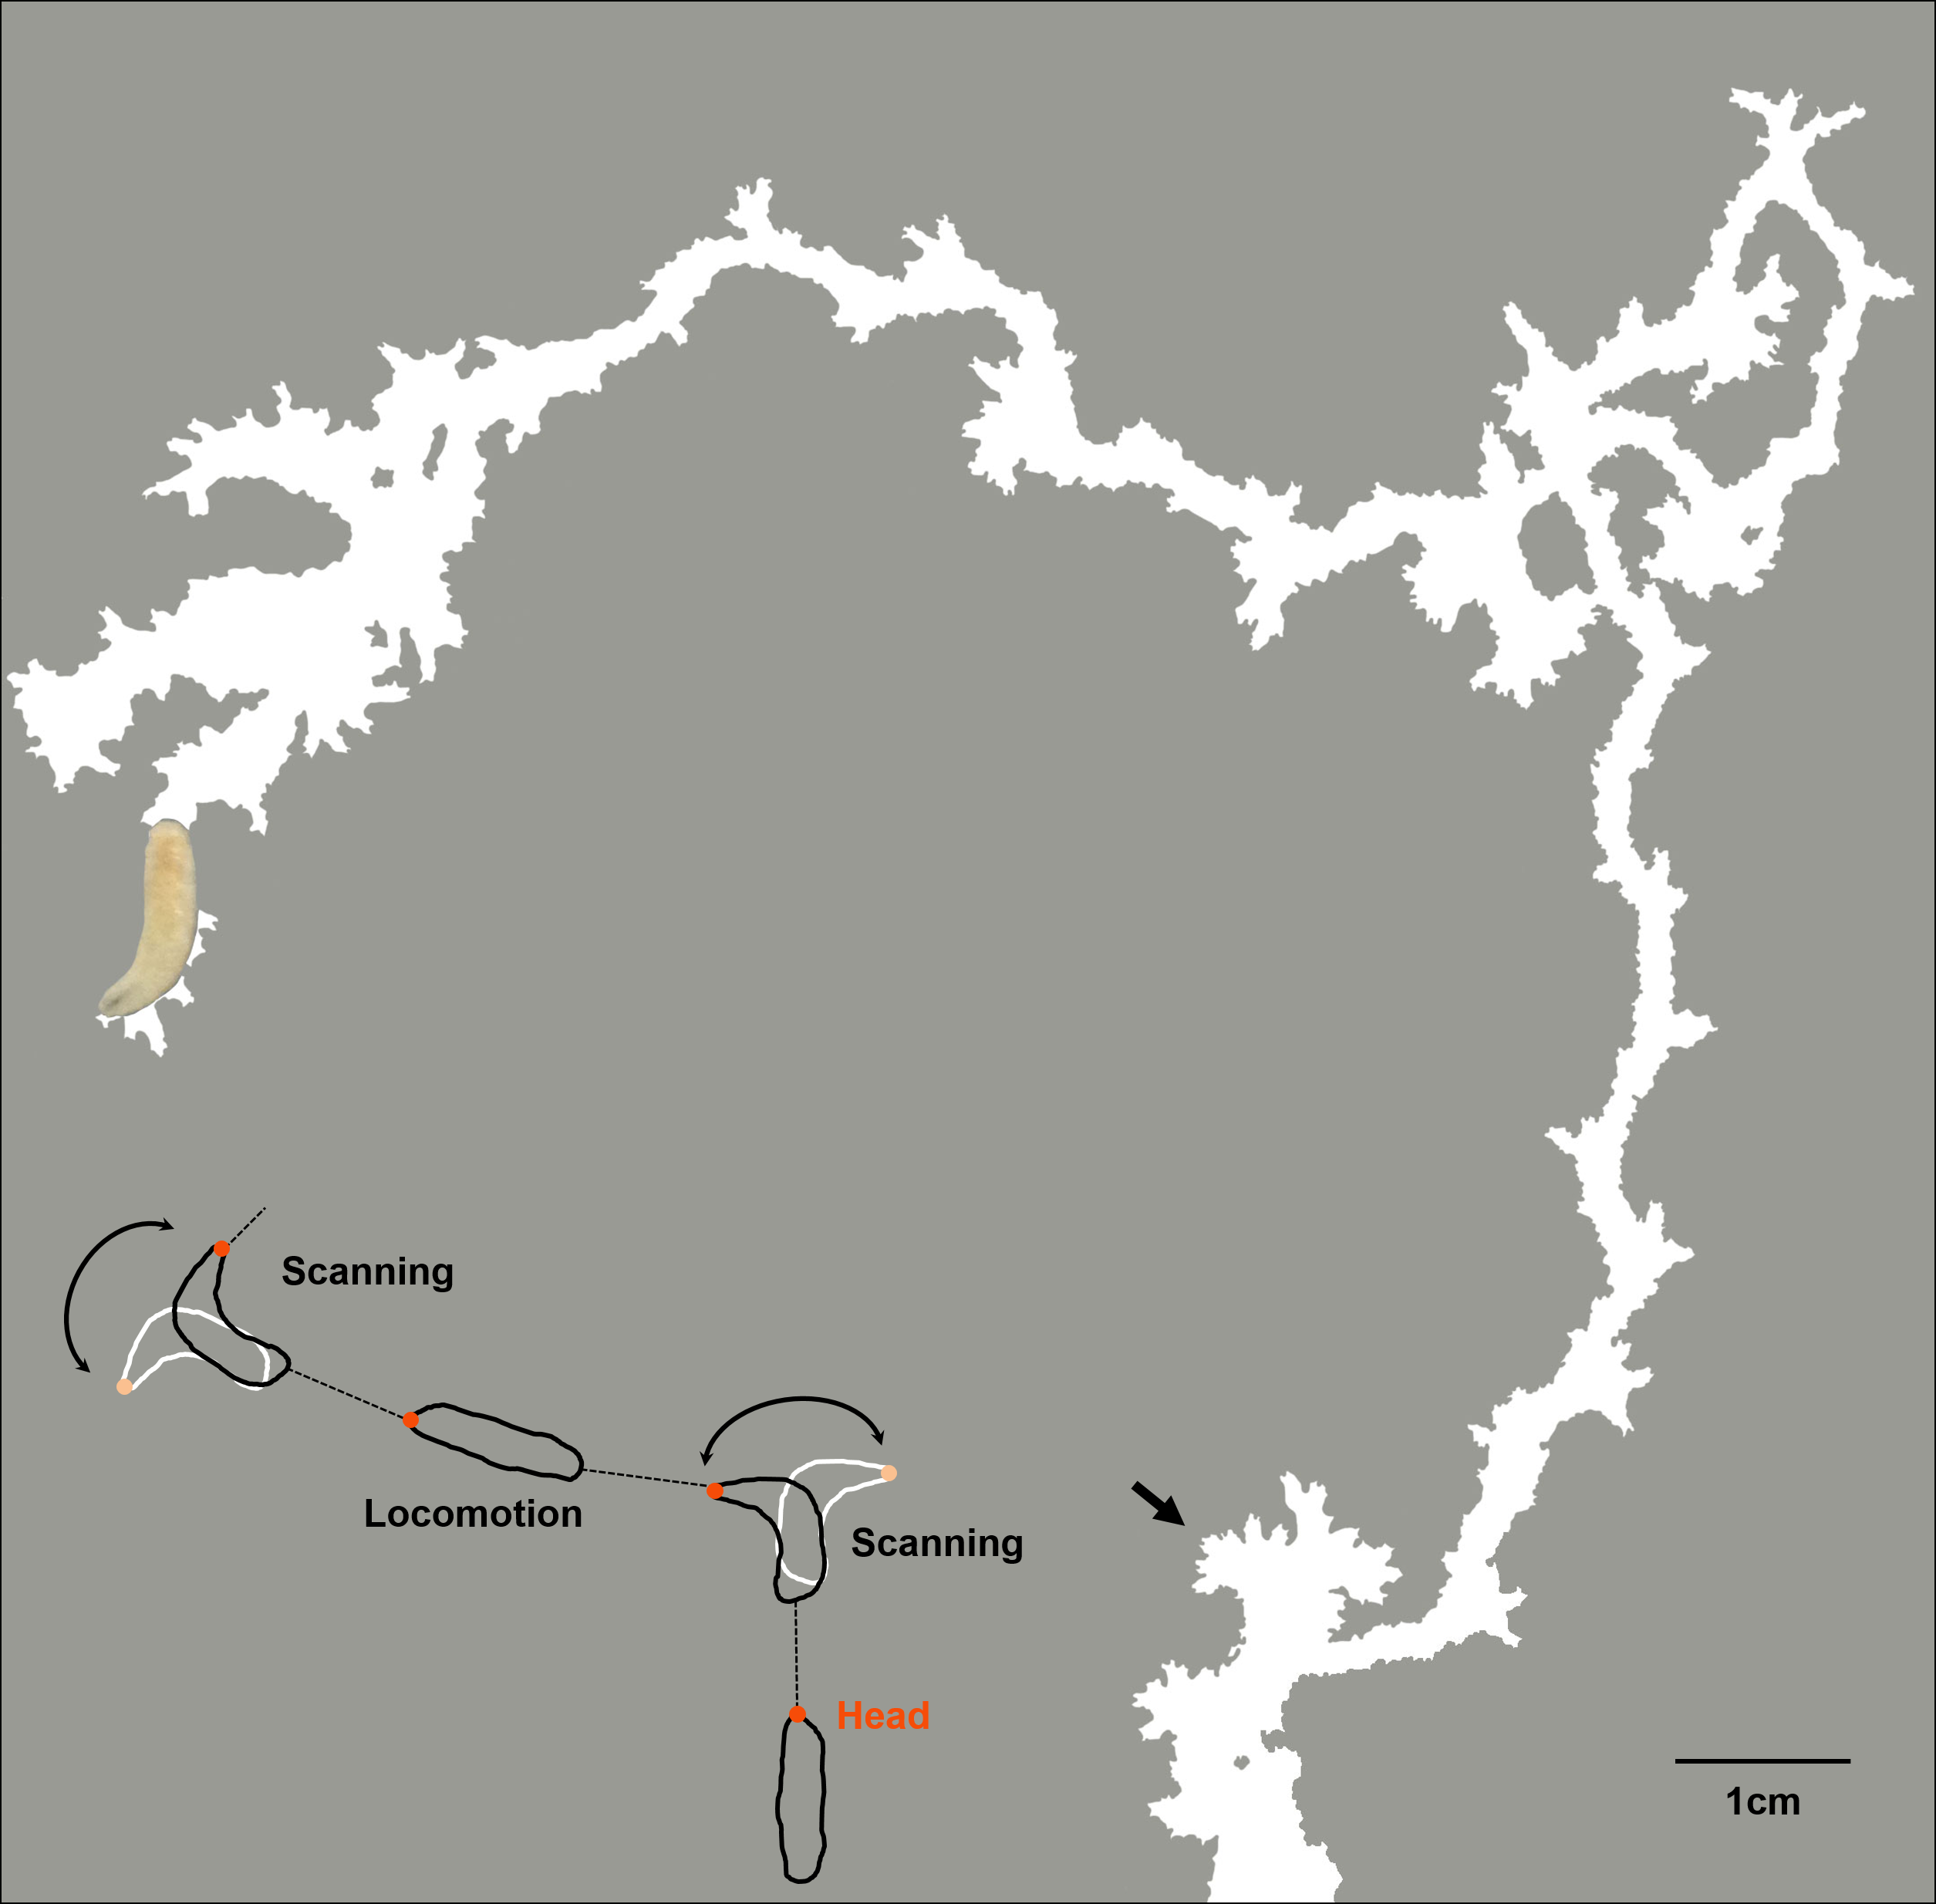
\includegraphics[width=0.6 \textwidth]{Figures/fig5.png}
		\rule{35em}{0.5pt}
	\caption[Scan]{A scheme of locomotion and scanning behaviour of \textit{Lucilia sericata} larva. During scanning, also named \textit{bending} \cite{green_organization_1983}, the larva is at the stop and successively turns the anterior third of its body on right and left directions. After few seconds scanning is over, the larva moves in the chosen direction. In white, the path of one \textit{L. sericata} larva in a new environment. The picture (modified from a photo) shows in white the area of physical contact between the larva and the substrate. The black arrow point one place where scanning occurred, with successive head position drawing a tree-like structure. Larva is visible at the left of the picture.}
	\label{fig:scan}
\end{figure}             

\clearpage           
%----------------------------------------------------------------------------------------
%	SECTION 5
%----------------------------------------------------------------------------------------
	\section{Discussion}   
    
%----------------------------------------------------------------------------------------
%	SUBSECTION 1
%----------------------------------------------------------------------------------------   
			\subsection{Limitations of the study}   
The authors are aware that this study does not definitely prove the implication of larval signal and scanning in aggregation of presocial larval blow fly. However, from the results obtained, it is reasonable to assume that the trail-following abilities of the larvae and the retentive effect of the 'larval signal' are involved in the aggregation process. Furthermore, although the exact role of scanning is not proven, there is a clear link with the presence of larval signal strongly implying a role in the aggregation behaviour.            
            
%----------------------------------------------------------------------------------------
%	SUBSECTION 2
%----------------------------------------------------------------------------------------   
			\subsection{Larval trail}
This study was designed to analyse the detection of a conspecific signals (as yet unidentified) by the necrophagous larvae of the Green bottle blow fly \textit{L. sericata} and to explore their signal-following abilities. Firstly, the results demonstrate that \textit{L. sericata} larvae are able to detect the boundaries of a signal left by conspecifics and their preference to stay within the prescribed area.  In the absence of signal from conspecifics, larval trajectories are straight with no about-turns. However, the prior presence of conspecifics (i.e., larval signal) impacts on the larval behaviour (Figure \ref{fig:trail}). Their trajectories are more sinuous, with numerous turns: larvae explore the arena instead of moving out of it (Figure \ref{fig:trail}). Accordingly, the \textit{L. sericata} larvae are able to detect a signal formerly left by conspecifics and alter their locomotion accordingly. A similar behaviour, based on biased running (very sinuous trajectories), has been observed during chemotaxis in Drosophila larvae \citep{gomez-marin_active_2011, gomez-marin_active_2012, ohashi_novel_2014}. This strategy is confirmed by regarding the branching tree-like path of \textit{L. sericata} larvae during an environment exploration (Figure \ref{fig:scan}). Larvae scan at each stop, turn slightly and continue their movement. The larvae are acquiring information about their environment (e.g., chemical gradient detection) by scanning, and are then moving accordingly.            
%----------------------------------------------------------------------------------------
%	SUBSECTION 3
%----------------------------------------------------------------------------------------   
			\subsection{Scanning behaviour}
The results show that \textit{L. sericata} larvae scan similarly in Control and Food conditions, but significantly less when a larval signal is present (Figure \ref{fig:proportion}). In both Control and Food conditions, the larval signal is absent: under these conditions, the larvae scan many times, and their successive scannings are close in time to each other. Such a scanning pattern is visible in Figure \ref{fig:scan}, which illustrates the result of numerous scans and changes in orientation. This finding agrees with that of \citet{green_organization_1983}, who observed no difference in the scanning frequency (called ‘bending’ in their study) of larval \textit{Drosophila melanogaster} between the food and no-food environments. On the other hand, individuals tested under Larvae and Larvae + Food conditions in the present study were directly in contact with the larval signal. They scanned for less time and less often. Accordingly, it is reasonable to assume that in \textit{L. sericata} larval scanning is involved in the detection of the chemical signal deposited by conspecifics on or in the substrate (i.e. klinotaxis; \citep{fraenkel_orientation_1961, gomez-marin_active_2012}). Further experiments will be required to identify the chemical composition of the larval signal (using gas-chromatography), and the involvement of the compounds identified in conspecific recognition (using behavioural tests). 

Aggregation of blow fly larvae is maintained by an active behaviour that is likely supported by a larval signal \cite{boulay_evidence_2013}. The detection of conspecific cues (tactile and chemical) is essential for larvae to be able to (re)join the group and to benefit from aggregation advantages \cite{rivers_physiological_2011}. The results presented here suggest that larvae use the scanning behaviour not only for turning but also to compare ground signals on either side (klinotaxis) and to orientate accordingly \cite{fraenkel_orientation_1961}. Larval masses are self-organized systems. One of the mechanisms of such social organization is the additive action of a signal that permits amplification of the system \cite{camazine_self-organization_2001}. According to the present observations and results, it is reasonable to conclude that scanning could be used by individual \textit{L. sericata} larvae to follow the trails left by conspecifics and/or to locate the most crowded areas. However, a precise description of the sensory organs of \textit{L. sericata} larvae and a demonstration of a direct linkage between these structures and the larval signal chemodetection are still needed. Such a linkage has already been explored for larvae of other dipteran species, such as \textit{Musca domestica} \citep{chu-wang_fine_1971, chu-wang_fine_1972}, \textit{Drosophila melanogaster} \cite{oppliger_neurophysiological_2000} and \textit{Hylemia sp.} \cite{honda_ultrastructures_1987}. 

%----------------------------------------------------------------------------------------
%	SECTION 6
%----------------------------------------------------------------------------------------
	\section{Acknowledgments}   
The authors would like to thank the two anonymous reviewers for their detailed and helpful suggestions. Authors also thank C. Devigne and J.L. Deneubourg (Senior Research Associate from the F.R.S.-FNRS) for their comments and M. Lemoine for photo editing.

\clearpage
    
    
            
            
            
